\documentclass[10pt]{beamer}

\usetheme{Montpellier}
\usecolortheme{beaver}

\usepackage{lmodern}
\usepackage{mathtools}
\usepackage{amsmath}
\usepackage{listings}
\usepackage{mdframed}
\usepackage{xcolor}
\usepackage{parskip}
\usepackage{substr}
\usepackage{hyperref}
\usepackage{etoolbox}
\usepackage{tipa}
\usepackage{pdfpages}
\usepackage{multicol}
\usepackage{cprotect}
\usepackage{booktabs}
\usepackage{silence}
\usepackage[backend=biber, style=ieee]{biblatex}
\usepackage[english,ngerman]{babel}
\usepackage{csquotes}
%\hypersetup{colorlinks = true, urlcolor=blue, linkcolor=white}
\mode<presentation>{}
\beamertemplatenavigationsymbolsempty
\setbeamertemplate{footline}[frame number]
\setbeamercolor{title in head/foot}{fg=black}
\setbeamercolor{subsection in head/foot}{fg=black}



\WarningFilter{biblatex}{Patching footnotes failed}

\renewcommand*{\bibfont}{\tiny}

\bibliography{resources.bib}

\titlegraphic{
\includegraphics[keepaspectratio, height=0.15\textheight]{img/logo_hertie.png} \\ [1em] 
\includegraphics[keepaspectratio, height=0.1\textheight]{img/logo.png}}

\title{\textbf{MEA LFP Analysis Toolbox}}
\author{\vspace{-0.7cm}F. Klopfer}
\date{\today}

\begin{document}
\frame{\titlepage}

\section{Introduction}
\begin{frame}
\begin{center}
 \begin{Huge}
  \textbf{Introduction}
 \end{Huge}
 \end{center}
\end{frame}

\begin{frame}[allowframebreaks]{Epilepsy \& Migraine as Channelopathies}
    \begin{center}
  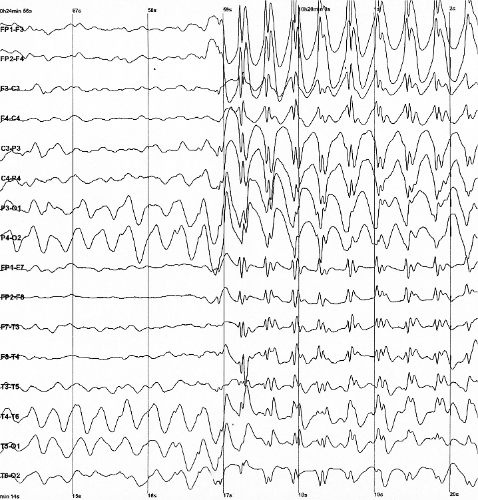
\includegraphics[keepaspectratio,width=0.48\framewidth]{img/0_channelo_epilepsy_eeg.png}
    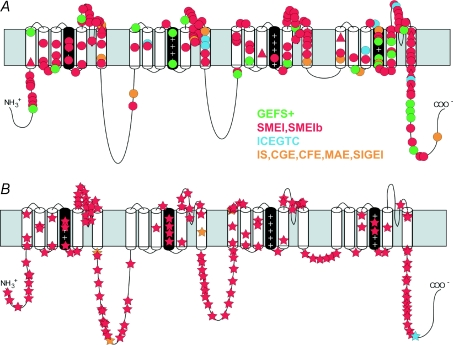
\includegraphics[keepaspectratio,width=0.48\framewidth]{img/0_channelo_nav11.jpg}

 \end{center}
 \framebreak
     \begin{center}
  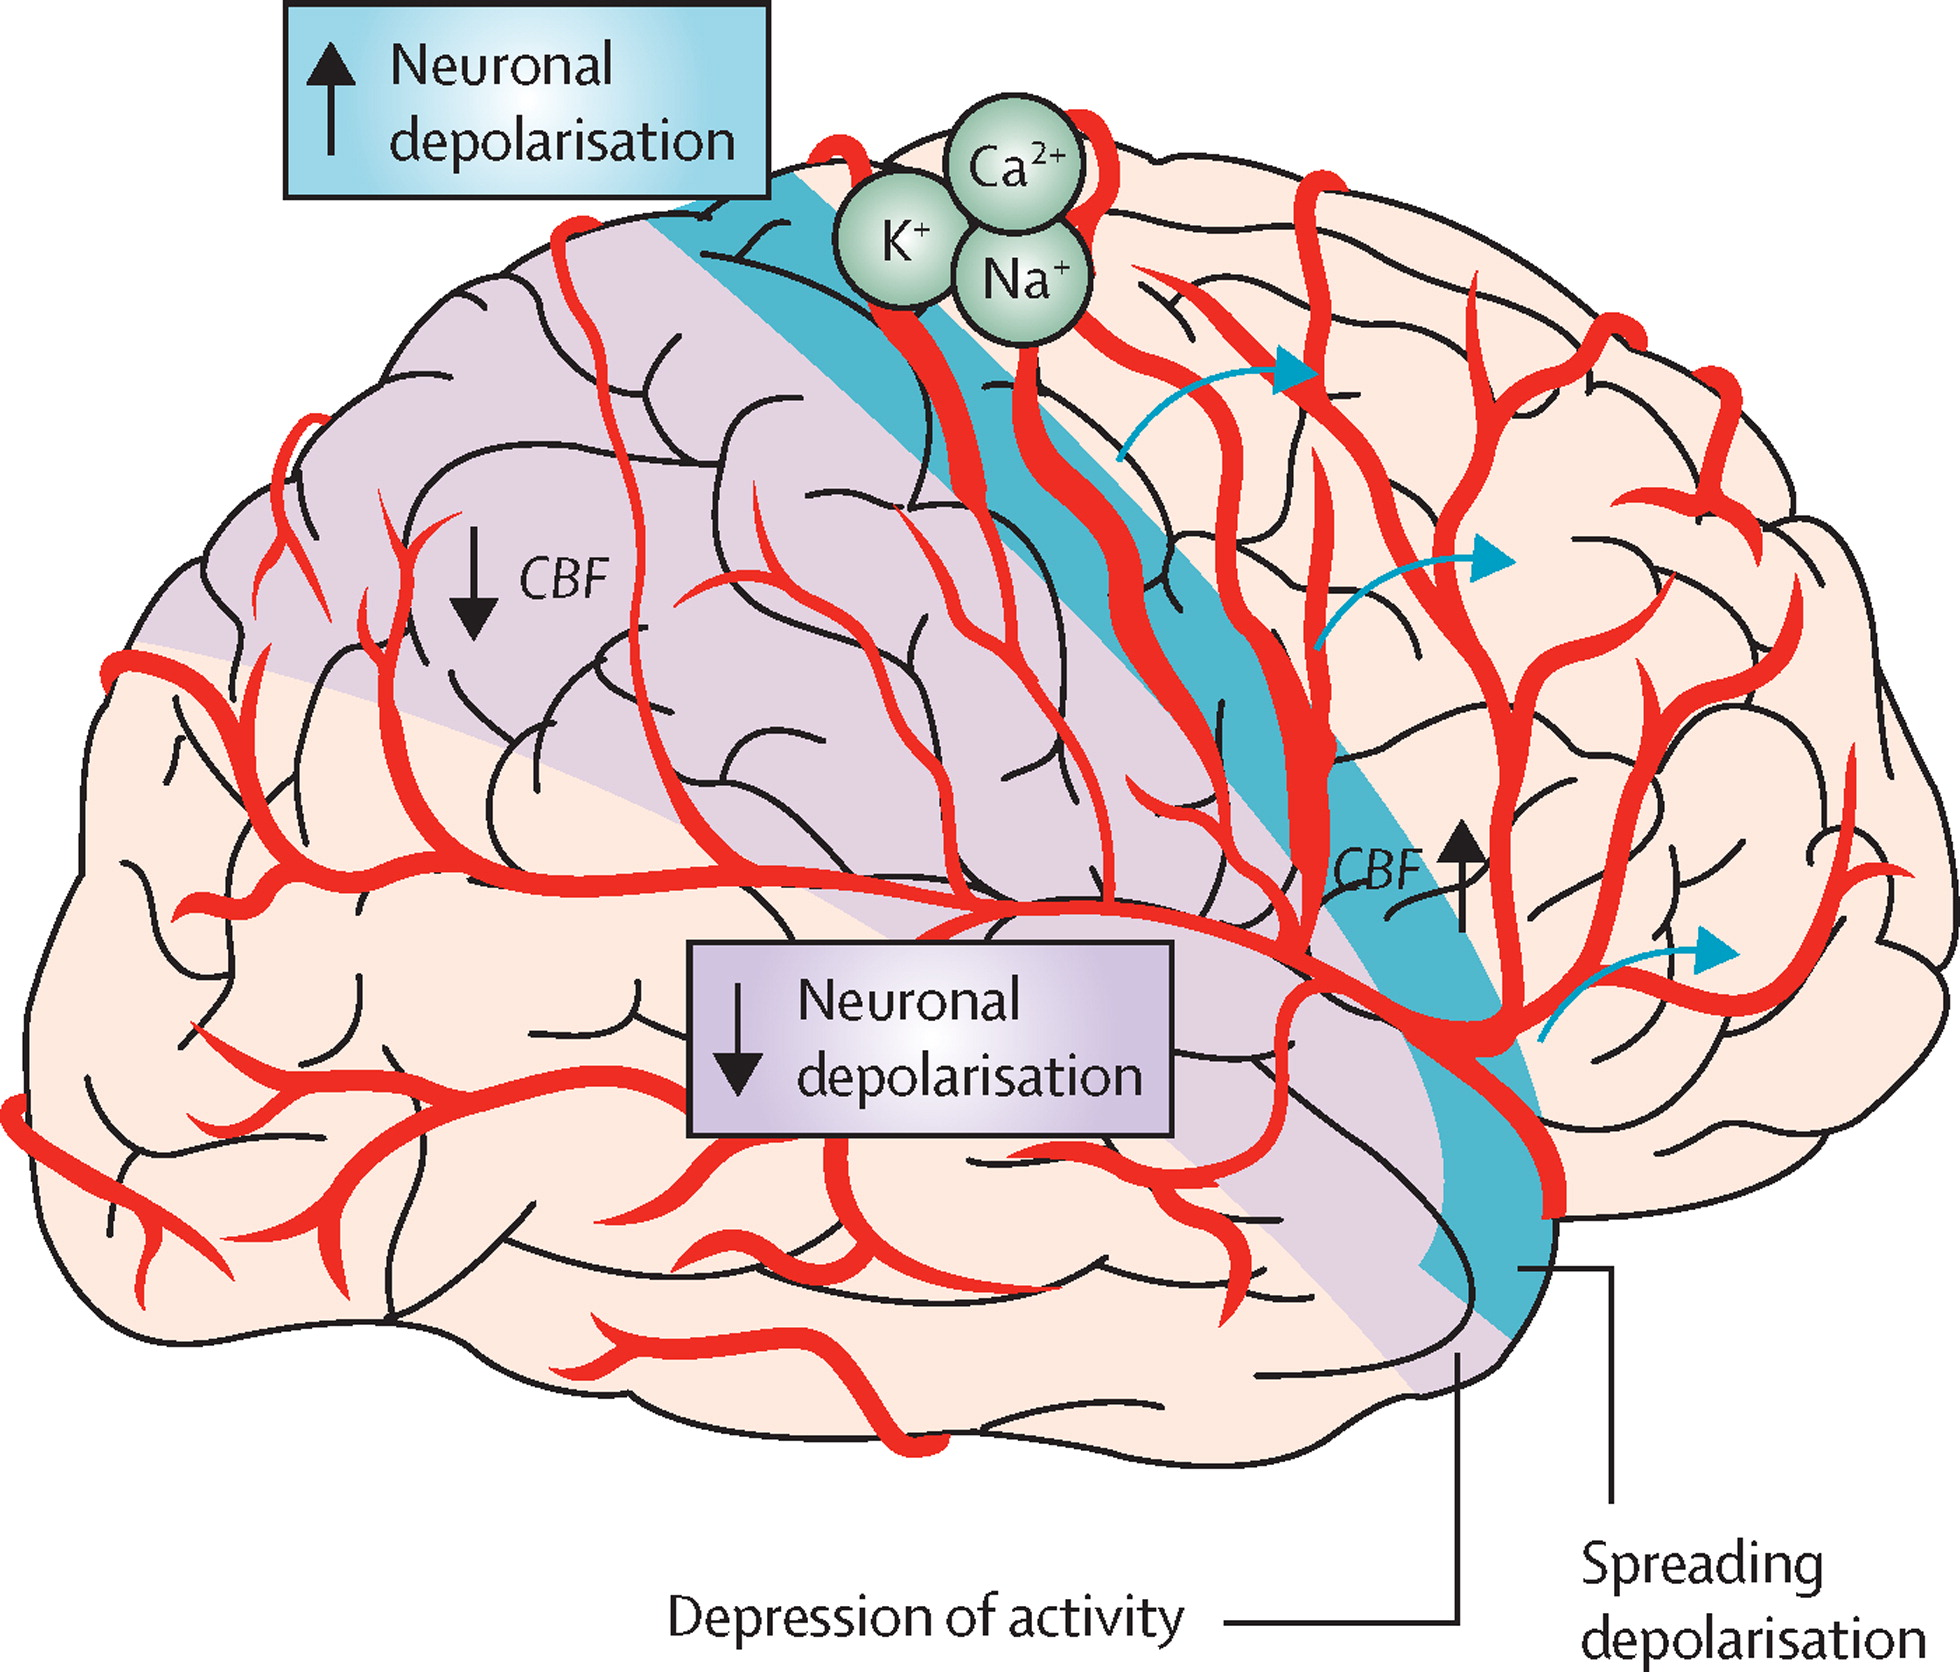
\includegraphics[keepaspectratio,width=0.38\framewidth]{img/0_channelo_migraine.jpg}
  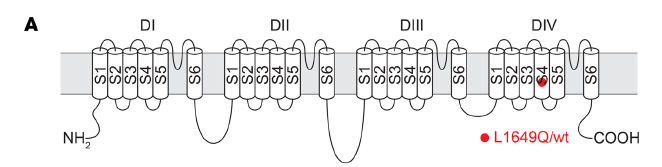
\includegraphics[keepaspectratio,width=0.58\framewidth]{img/0_channelo_nav11_mig.png}
 \end{center}
\end{frame}


\begin{frame}[allowframebreaks]{Recording Setup}
  \begin{center}
  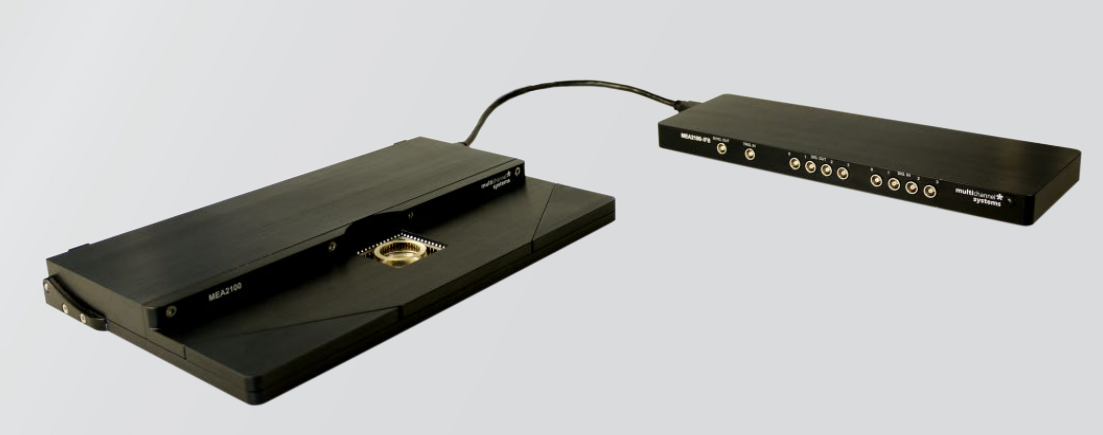
\includegraphics[keepaspectratio,width=0.95\framewidth]{img/1_setup_mea.png}
 \end{center}
 \framebreak
 \begin{center}
  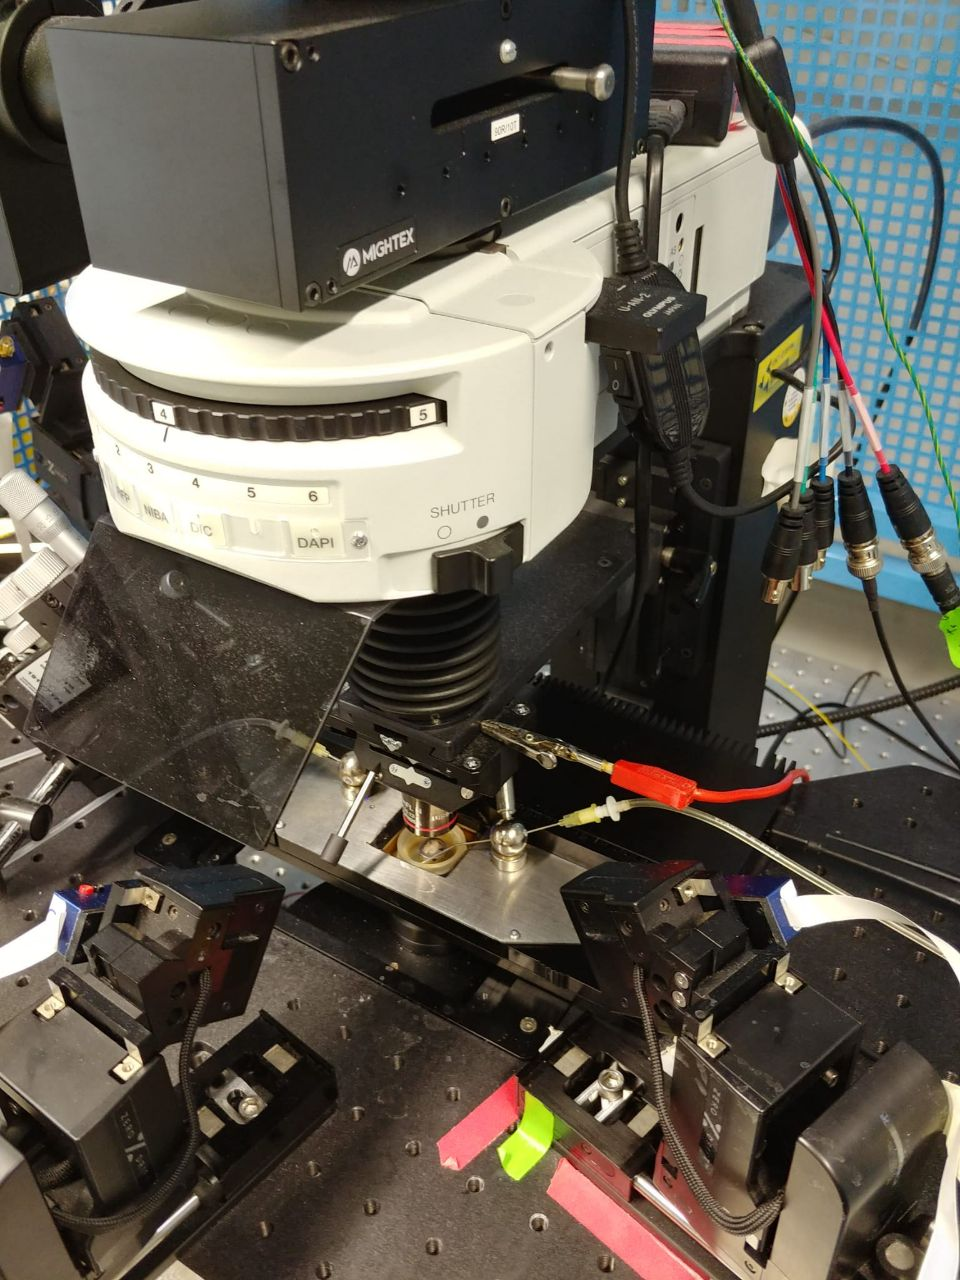
\includegraphics[keepaspectratio,width=0.47\framewidth]{img/1_setup_top.jpg}
   \end{center}
 \framebreak
 \begin{center}
    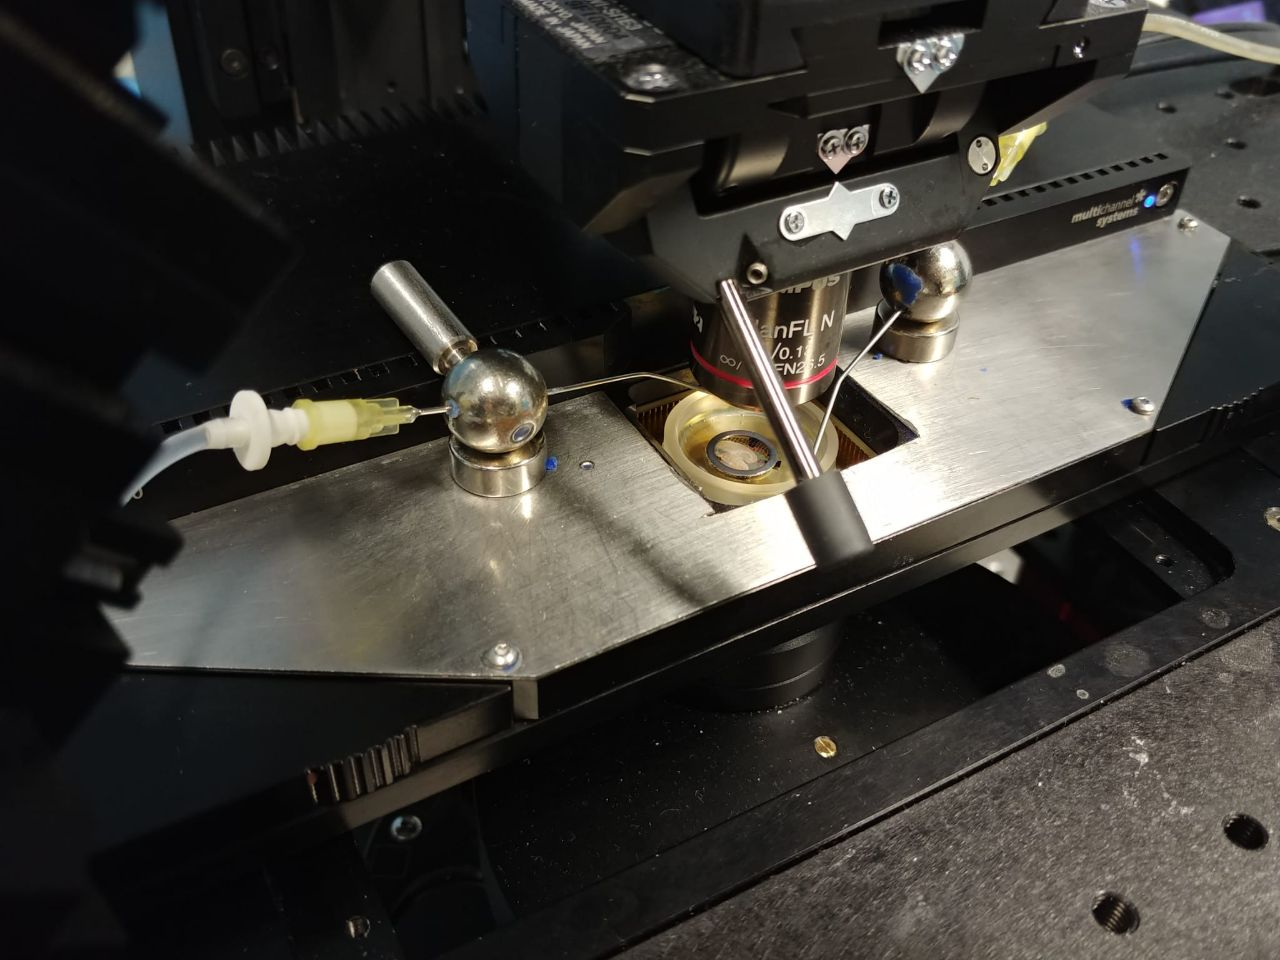
\includegraphics[keepaspectratio,width=0.8\framewidth]{img/1_setup_close.jpg}
 \end{center}
  \framebreak
 \begin{center}
  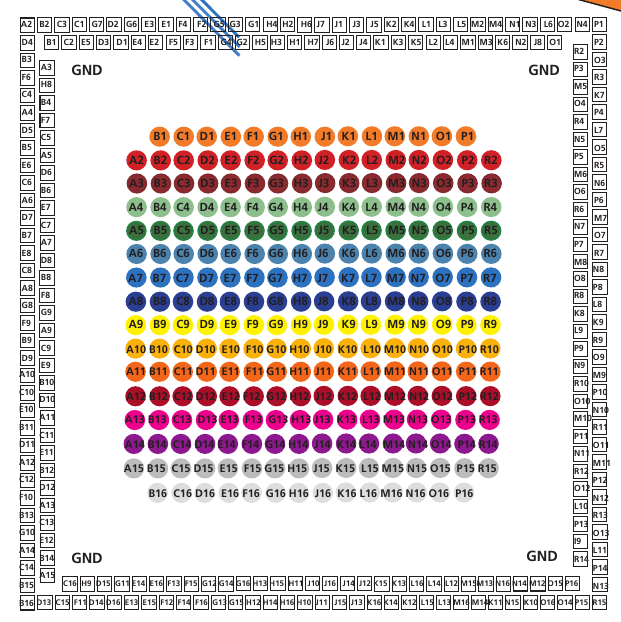
\includegraphics[keepaspectratio,width=0.6\framewidth]{img/1_setup_mea_layout.png}
   \end{center}
  \framebreak
 \begin{center}
    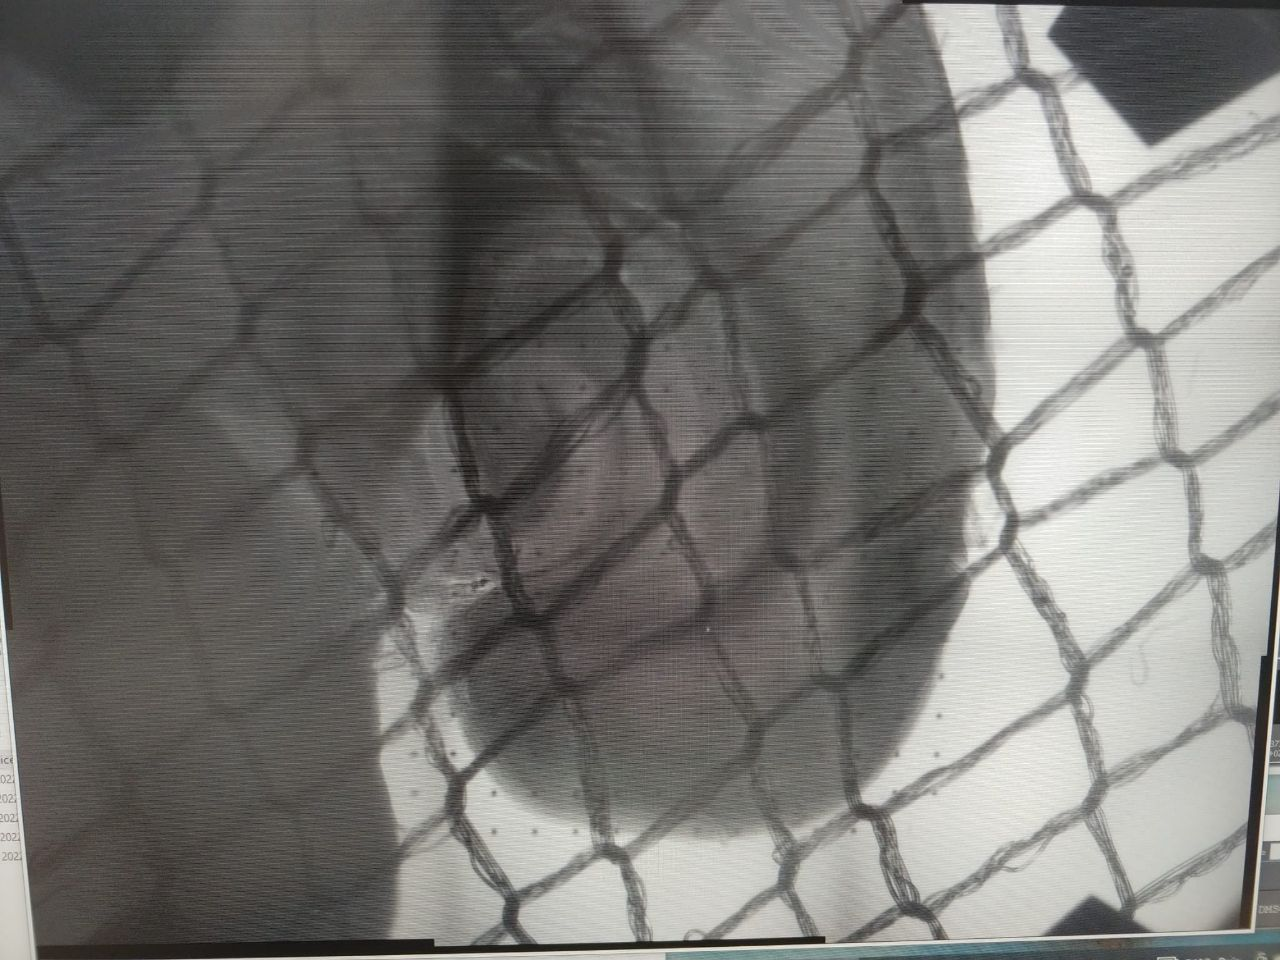
\includegraphics[keepaspectratio,width=0.9\framewidth]{img/1_setup_slice_.jpg}

 \end{center}
\end{frame}

\begin{frame}[allowframebreaks]{Data}
\begin{center}
  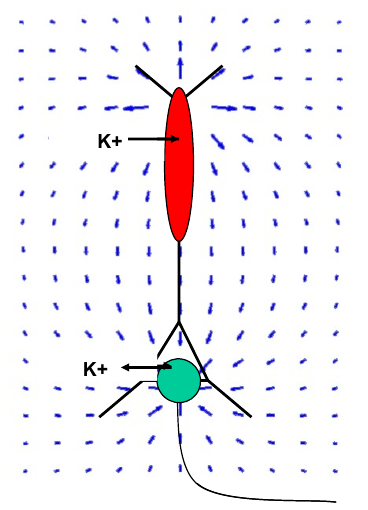
\includegraphics[keepaspectratio,width=0.35\framewidth]{img/2_lfp.png}
  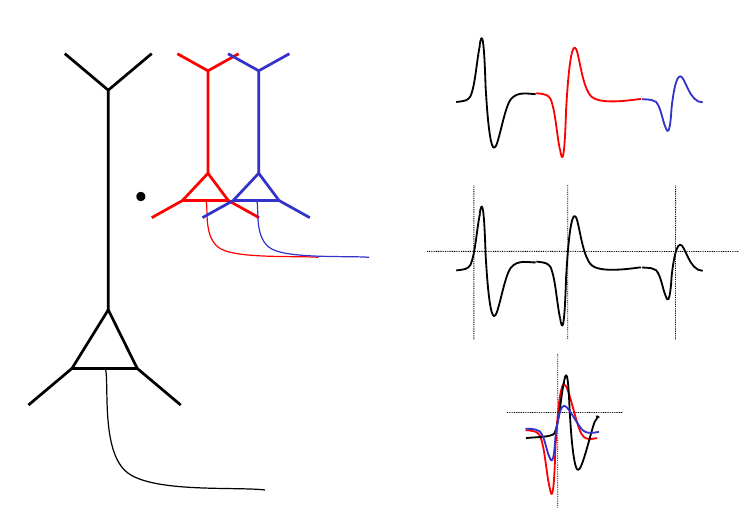
\includegraphics[keepaspectratio,width=0.64\framewidth]{img/2_lfp_mur.png}
 \end{center}
 \framebreak
 \begin{center}
  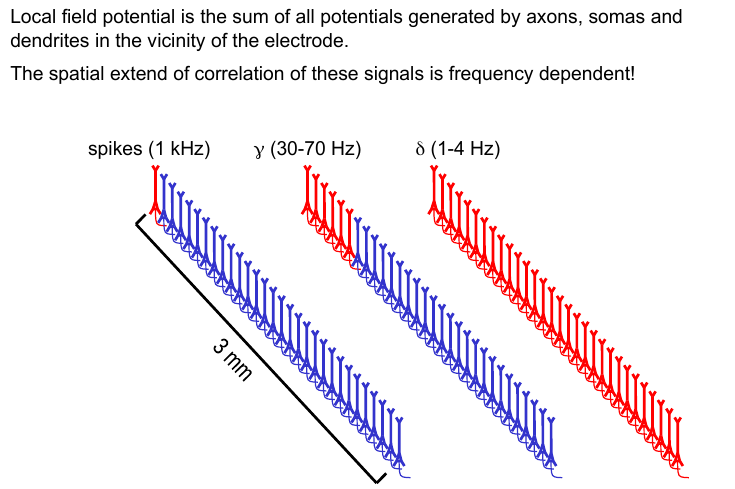
\includegraphics[keepaspectratio,width=0.8\framewidth]{img/2_lfp_origins.png}
 \end{center}
  \framebreak
 \begin{center}
  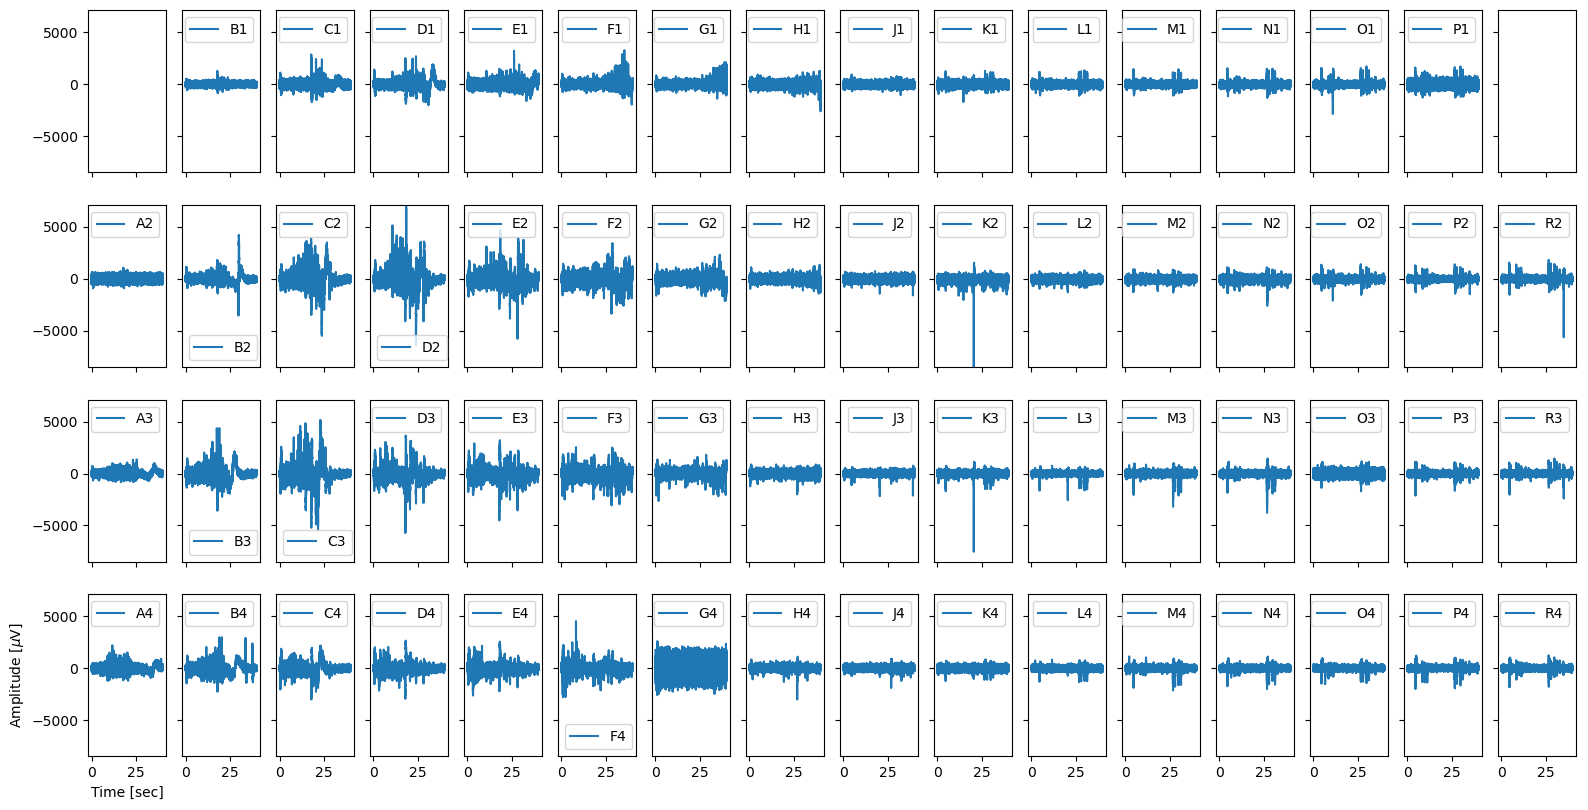
\includegraphics[keepaspectratio,width=\framewidth]{img/4_raw.png}
 \end{center}
\end{frame}

\begin{frame}{Task}
\begin{itemize}
 \item Task: Detect peaks, seizure-like bursts \& characterize them. Provide GUI. \\ [2em]
 \item Contraints: \begin{itemize}
                    \item many channels \\ [1em]
                    \item high sampling rate \\ [1em]
                    \item high heterogeneity \\ [2em]
                   \end{itemize}
  \item Existing toolboxes are
  \begin{itemize}
   \item proprietary or vendor specific
   \item scale specific (Single Unit vs. EEG/MEG)
   \item quality-wise insufficient
  \end{itemize}
\end{itemize}
\end{frame}

\section{Software}
\begin{frame}
\begin{center}
 \begin{Huge}
  \textbf{Software}
 \end{Huge}
 \end{center}
\end{frame}


\begin{frame}[allowframebreaks]{MEA LFP Analysis Toolbox}
    Semi-automated data analysis pipeline with UI. \\ [1em]
    \begin{itemize}
     \item Currently supports MultiChannel Systems 256 electrode MEA \\ [1em]
      \begin{center}
        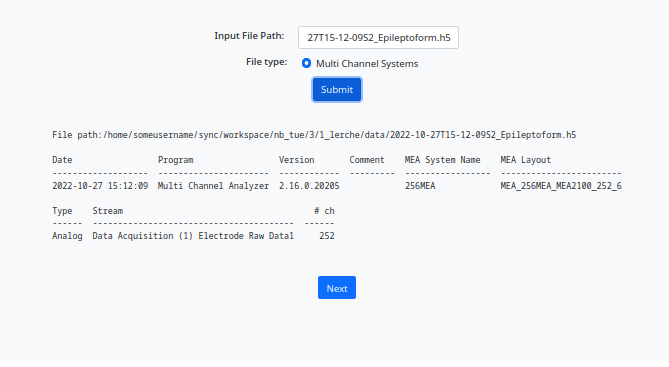
\includegraphics[keepaspectratio,width=0.8\framewidth]{img/4_import.png}
      \end{center}
      \framebreak
      
     \item Allows graphical selection of electrodes and time window \\ [1em]
      \begin{center}
        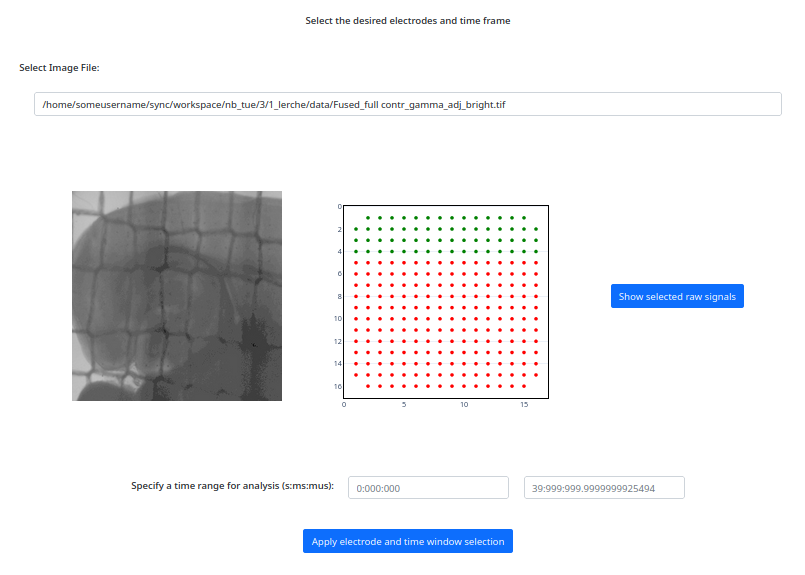
\includegraphics[keepaspectratio,width=0.8\framewidth]{img/4_select.png}
      \end{center}
      \framebreak
      
     \item Preprocessing: Electrical humming filter, bandpass filter, downsampling \\ [1em]
      \begin{center}
        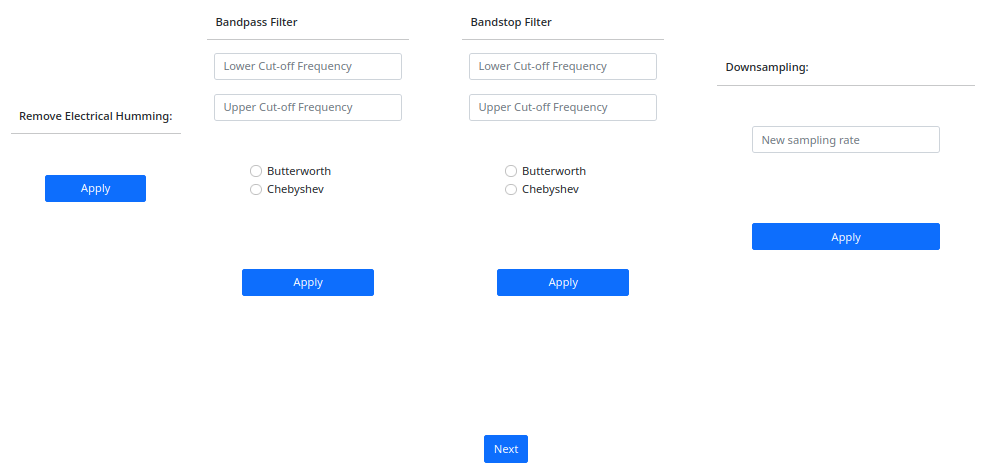
\includegraphics[keepaspectratio,width=0.8\framewidth]{img/4_preproc.png}
      \end{center} 
      \framebreak
      
     \item Exploration: raw signal plots, absolute amplitude video, PSD, Spectrogram \\ [1em]
      \begin{center}
        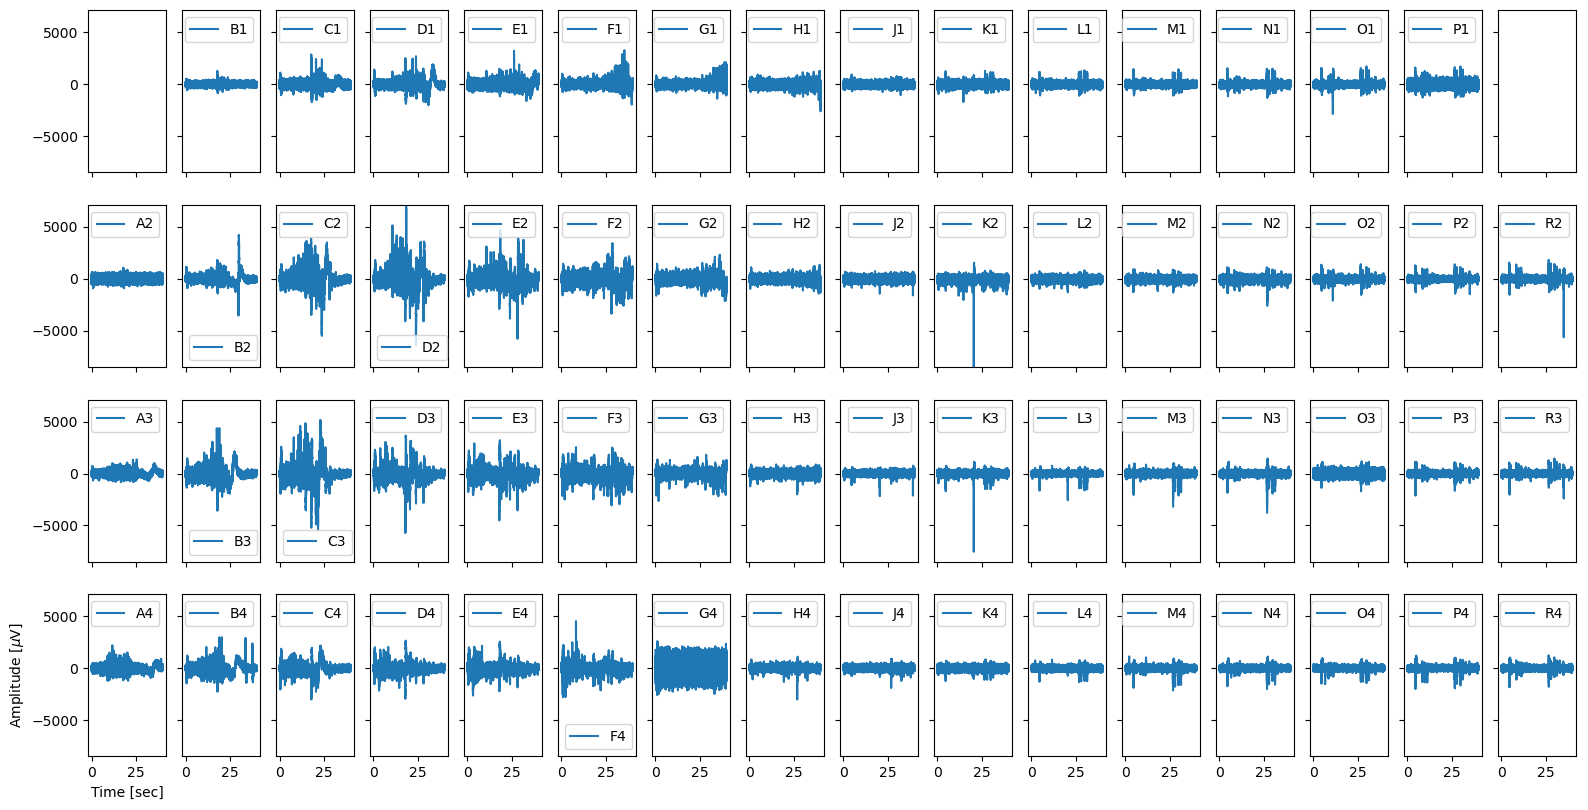
\includegraphics[keepaspectratio,width=0.9\framewidth]{img/4_raw.png}
      \end{center}
      \framebreak
      \begin{center}
        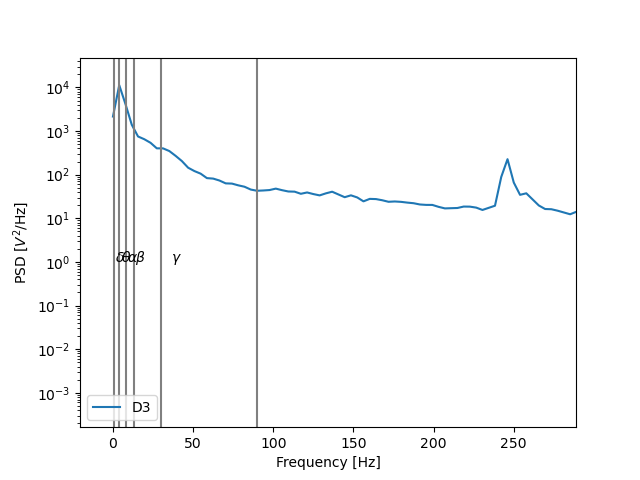
\includegraphics[keepaspectratio,width=0.8\framewidth]{img/4_psd.png}
      \end{center}
      \framebreak
      \begin{center}
        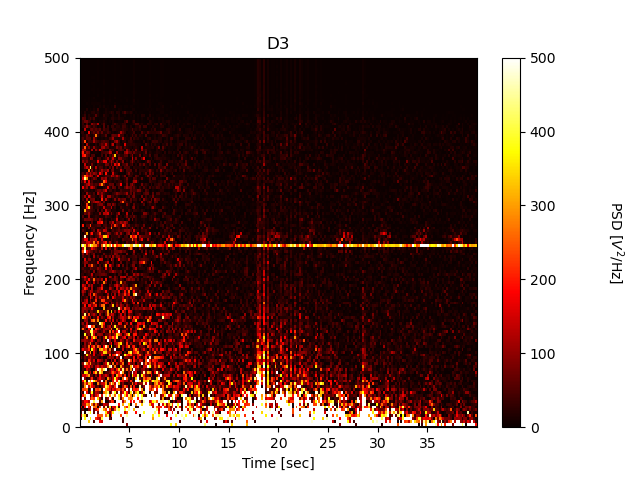
\includegraphics[keepaspectratio,width=0.8\framewidth]{img/4_spectrogram.png}
      \end{center}
      \framebreak
      
     \item Analysis: Peak detection based on theshold derived from std or based on moving average, burst detection based on moving average or moving std (instead of peaks) \\ [1em]
        \begin{center}
      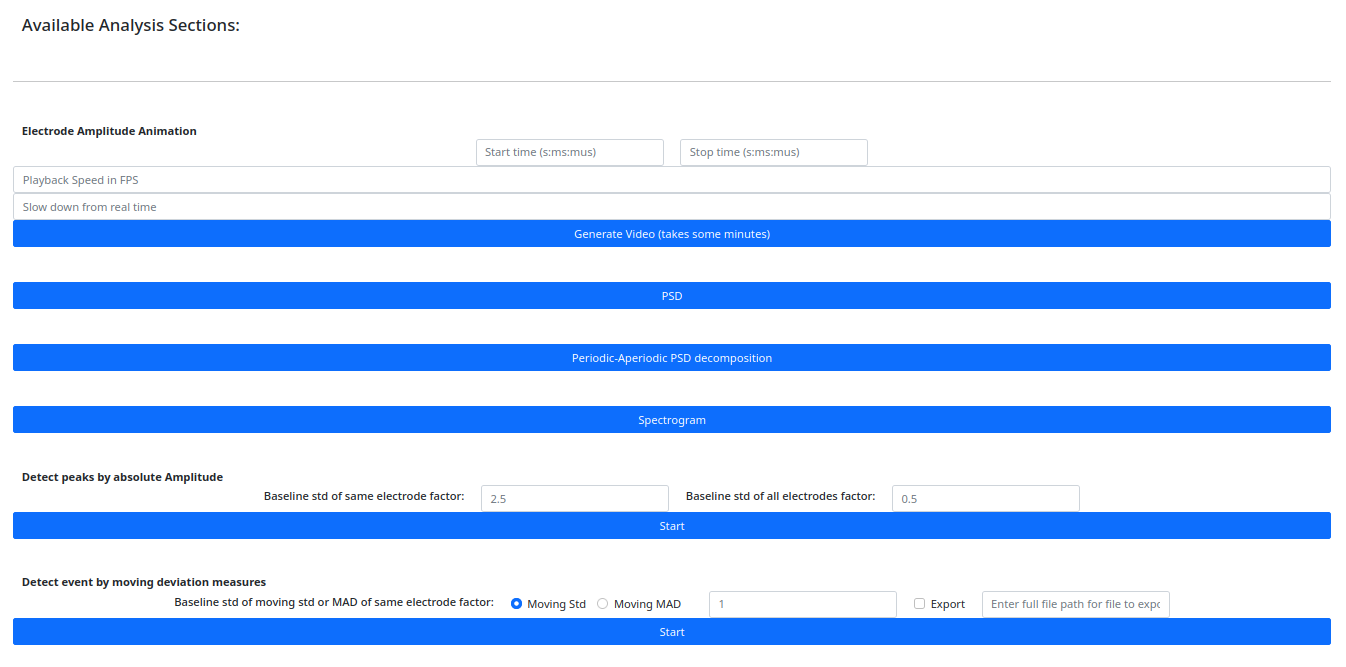
\includegraphics[keepaspectratio,width=0.8\framewidth]{img/4_analyze.png}
      \end{center}
      \framebreak
      \hspace{-1cm}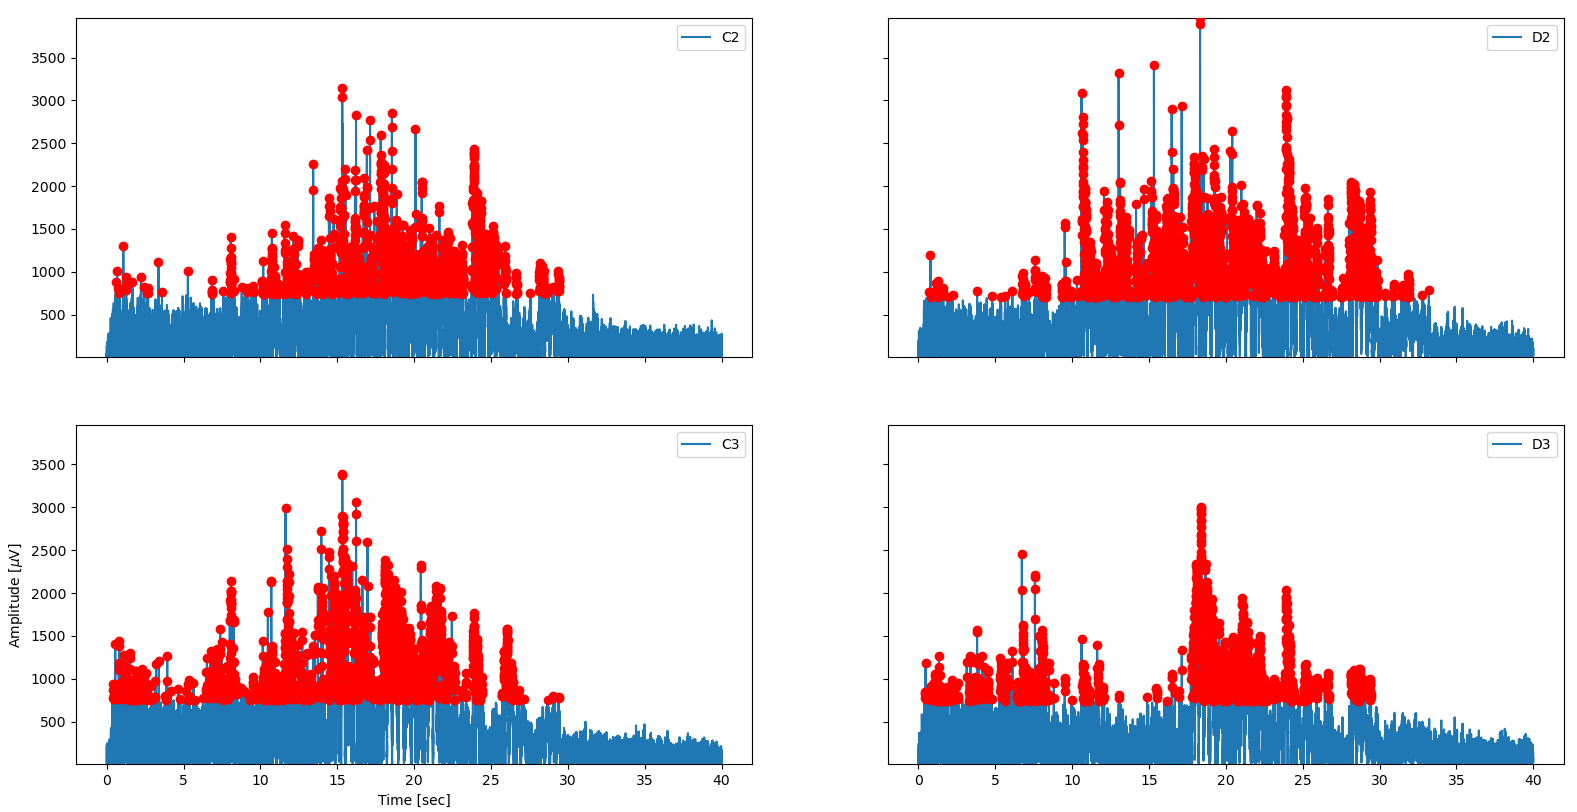
\includegraphics[keepaspectratio,width=\framewidth]{img/4_peaks_amplitude.png}
      \framebreak
      \hspace{-1cm}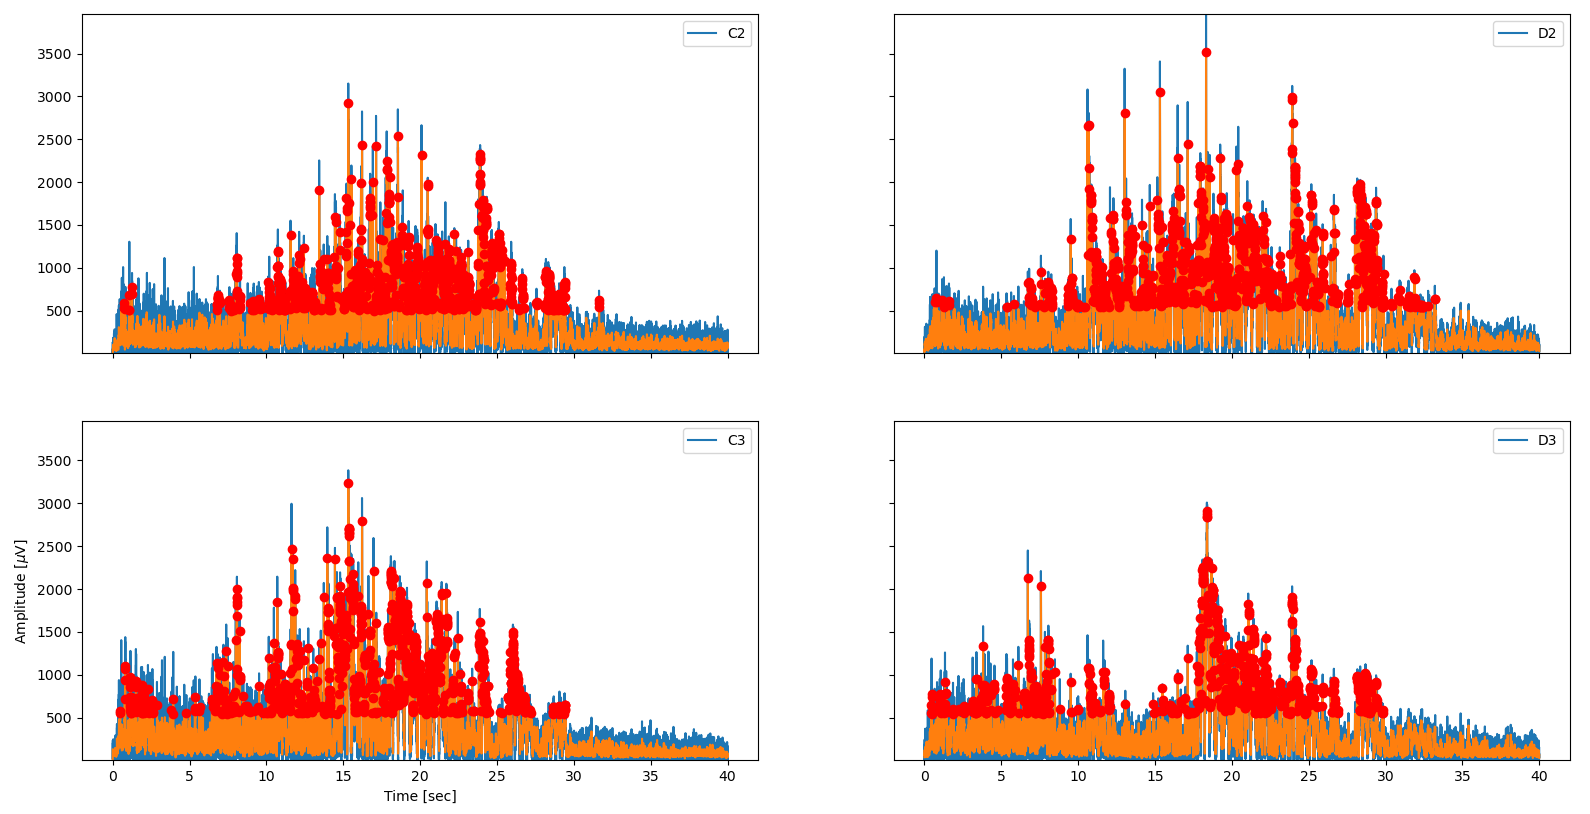
\includegraphics[keepaspectratio,width=\framewidth]{img/4_peaks_avg.png}
      \framebreak
      \begin{center}
      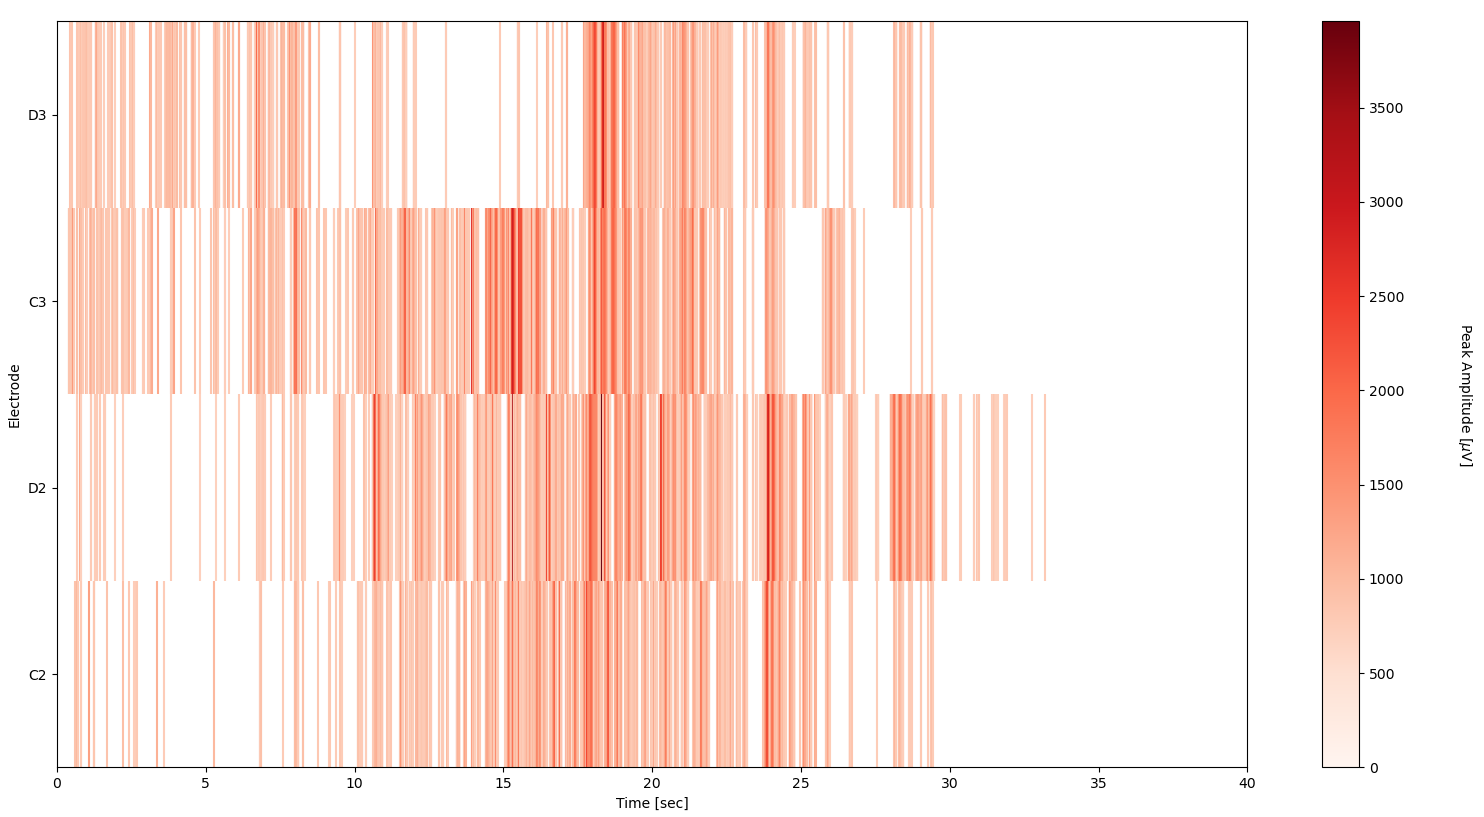
\includegraphics[keepaspectratio,width=0.58\framewidth]{img/4_raster_amplitude.png}
      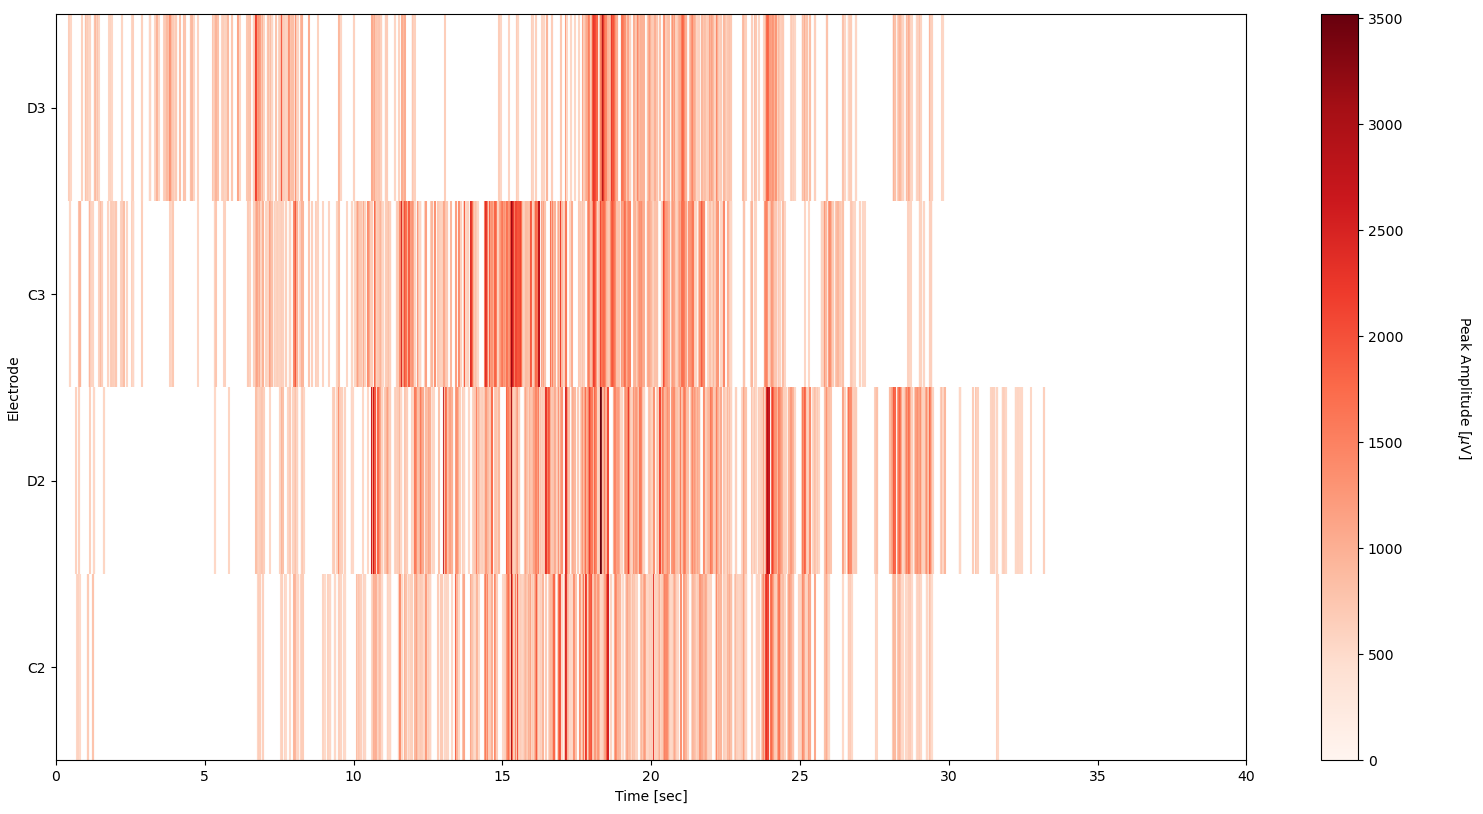
\includegraphics[keepaspectratio,width=0.58\framewidth]{img/4_raster_avg.png}
      \end{center}
      \framebreak
      
      \hspace{-1cm}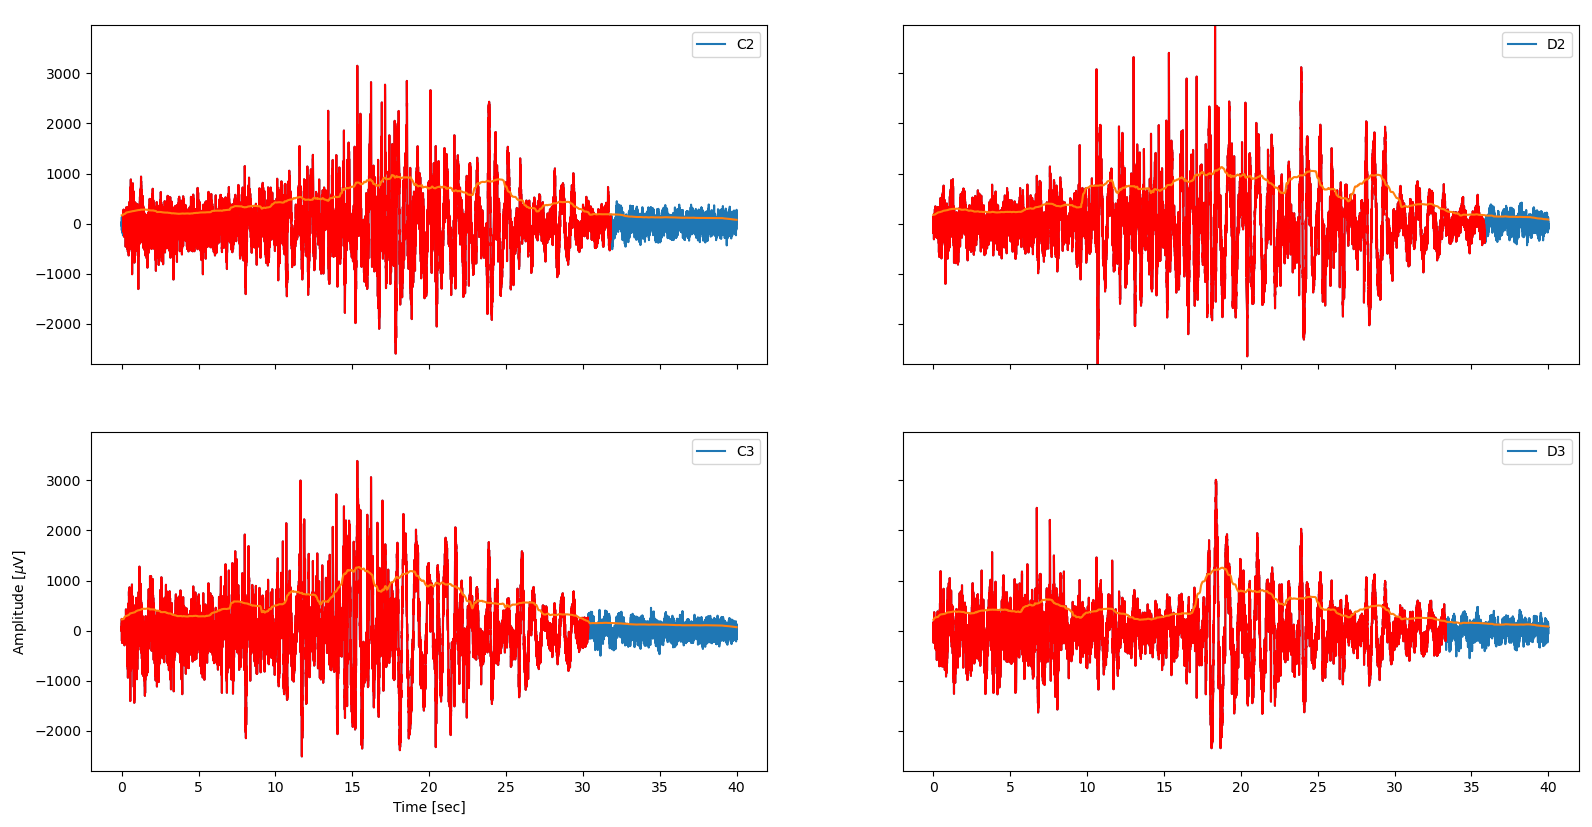
\includegraphics[keepaspectratio,width=\framewidth]{img/4_bursts_std.png} \\
      \hspace{-1cm}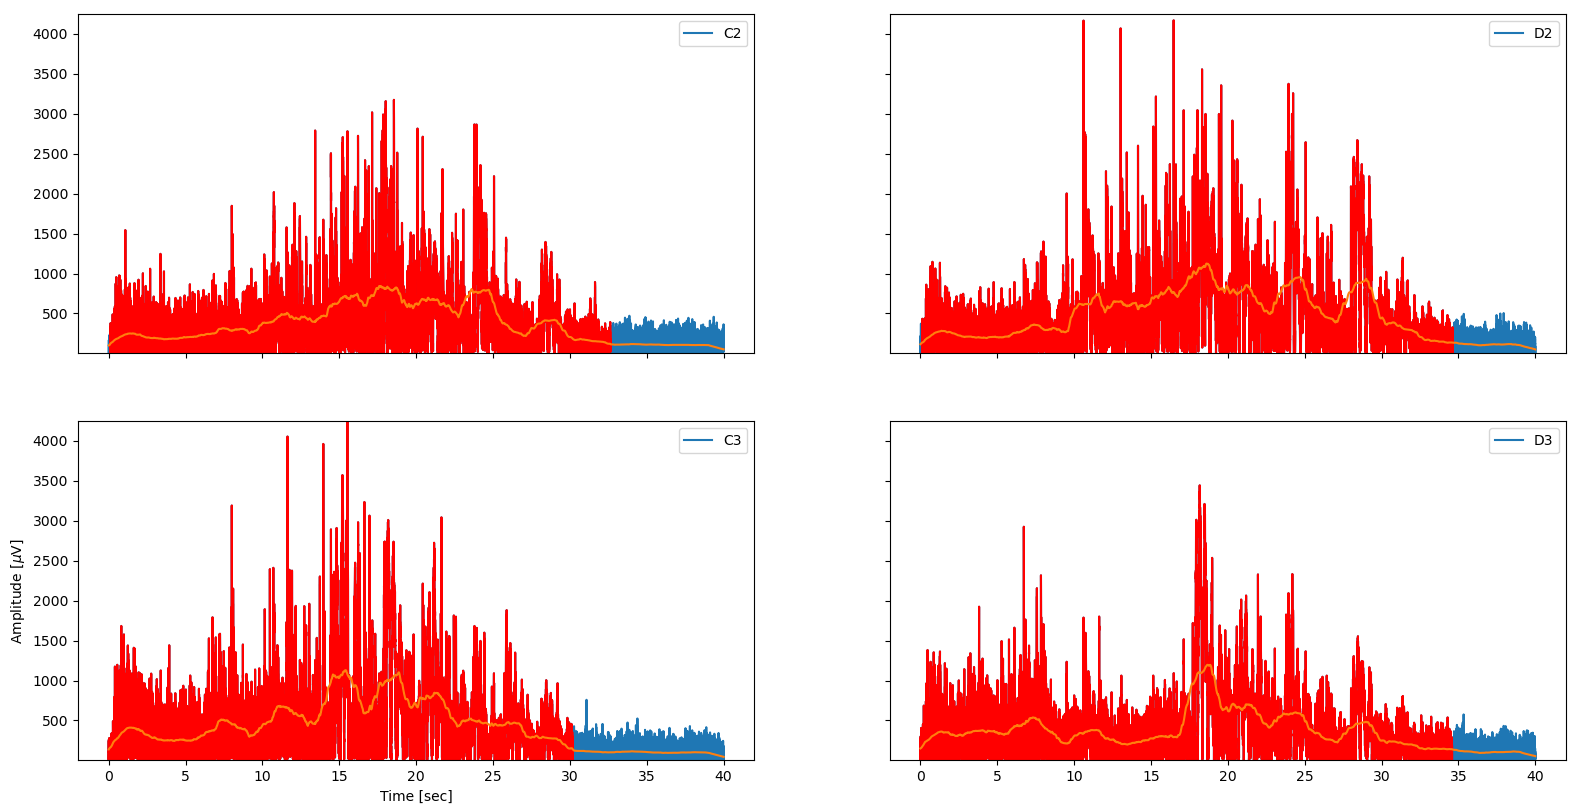
\includegraphics[keepaspectratio,width=\framewidth]{img/4_bursts_avg.png}
      \framebreak
      
     \item seizure-like event quantification: \\ 
      \hspace*{-1.5cm}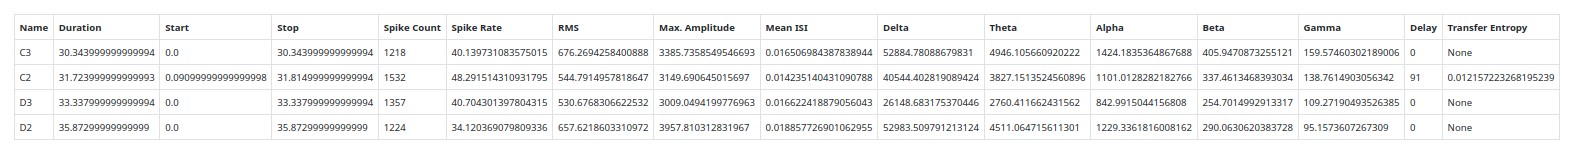
\includegraphics[keepaspectratio,width=1.1\framewidth]{img/4_event_stats_std.png} \\
      \hspace*{-1.5cm}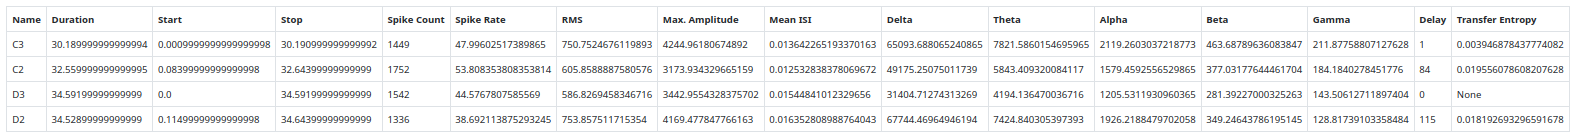
\includegraphics[keepaspectratio,width=1.1\framewidth]{img/4_event_stats_avg.png}
     \end{itemize}
     \end{frame}

\section{Outlook}
\begin{frame}
\begin{center}
 \begin{Huge}
  \textbf{Outlook}
 \end{Huge}
 \end{center}
\end{frame}

\begin{frame}{Outlook}
\begin{itemize}
 \item Transfer Entropy, Granger Causality and CSD \\ [1em]
 \item Group analysis \\ [1em]
 \item Other setups: CMOS, deep brain stimulation electrodes \\ [1em]
 \item in-vitro/MEA - in-vivo/Tetrode correlation \\ [1em]
 \item 2-Photon Ca$^{2+}$ imaging \\ [1em]
\end{itemize}
\end{frame}
     
     
\section{References}
    \begin{frame}[allowframebreaks]
      \frametitle{References}
      \begin{tiny}
      \nocite{*}
      \printbibliography
      \end{tiny}
    \end{frame}

 \end{document}
